\chapter{Análise Bibliográfica sobre Otimizações algorítmicas para simulações de fenômenos fluídos e óticos por Alexsander Correa de Oliveira}

\section{Planejamento do estudo}
    A indústria de jogos é a que mais cresce dentre todas as formas de entretenimento atuais. Alguns desses jogos podem chegar a investimentos tão grandes que disputam com os filmes mais caros da história. No posto de vista do consumidor, todo tempo e dinheiro gastos são apenas meios para um fim, que é o de ter a melhor experiência possível. Contudo do ponto de vista dos desenvolvedores, esses fatores são consequências de horas e horas de trabalho.
    
    Toda a tecnologia criada para esses jogos tem de ser cada vez mais eficiente, dado a necessidade de tornar os gráficos cada vez mais realistas, e seus mundos ainda mais acreditáveis. As técnicas utilizadas para tal otimização são fortemente baseadas em artigos \emph{state-of-the-art} tanto e física quanto em geometria.
    
    Entre todos aspectos físicos, que hoje em dia são mais prevalentes nos jogos, temos algumas áreas de estudo que pesam mais, principalmente em performance: 
    \begin{itemize}
        \item Corpos fluídos, como água e ar;
        \item Análise de vetores em ótica, para saber como a iluminação afetará um determinado ambiente;
        \item Análise da topologia, com fins de otimizar \emph{path-finding};
    \end{itemize}
\subsection{Uso do Bibliometrix e Biblioshiny}
     Com o auxílio das ferramentas disponibilizadas pelo Bibliometrix, como o Biblioshiny, serão analisados os artigos encontrados, por meio de gráficos e tabelas.   
\section{Coleta de Dados}
    A coleta de dados foi iniciada no dia 02/02/2022, e usou a base Web of Science, com acesso direto pelo periódico Capes.
    
    Por fins de diminuir o tamanho do \emph{dataset}, só foi utilizada a edição \emph{Science Citation Index Expanded}, que tem o foco voltado para ciências exatas e naturais.
    
    A busca inicial foi feita com a seguinte \emph{query}:
\begin{lstlisting}
((algorit* ) and (Optimization)) and 
(optics or ((fluid* or aero*) and dynamics))
\end{lstlisting}
\subsection{Explicação para a \emph{Query}}
    A busca foi feita com o objetivo de encontrar apenas técnicas para otimizar algoritmos relacionados a ótica, aerodinâmica e hidrodinâmica.
    
    Os termos $((algorit* ) and (Optimization))$ são para encontrar apenas os artigos relacionados a algoritmos computacionais.
    
    Já $(optics or ((fluid* or aero*) and dynamics))$ serve para falar que tanto faz um artigo de ótica ou de aerodinâmica ou de hidrodinâmica.
    
    Com a \emph{Query} já montada, os registros foram exportados do WoS com todas as informações disponíveis e no formato de arquivo de texto sem formatação. Foram recuperados desa maneira, 7443 registros no total.
\section{Análise dos dados}
    Uma análise inicial foi feita com o objetivo de retirar artigos indesejados. Para atingir isso, foi utilizado o gráfico \emph{Co-occurrence Network}, que mostra as palavras com maior peso, e o relacionamento entre elas.
    
     \begin{figure}
    \centering
    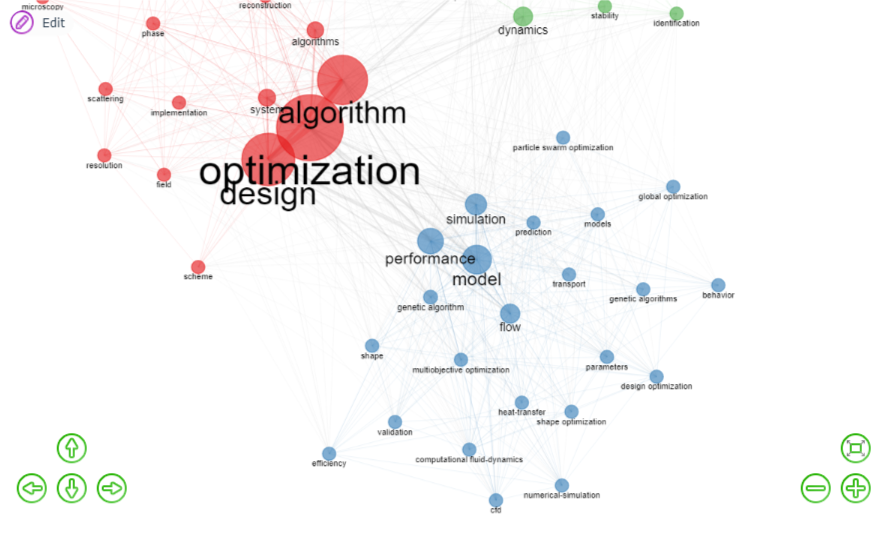
\includegraphics[width=1\textwidth]{experiments/KvotheKS/PesqBibliogr/AlgoritmosSimulacaoOptica-Dinamica/WoS-20220202/OldQueryDataset/CoOccurrence.png}
    \caption{Rede de co-ocorrência}
    \label{fig:KvotheKS:OldQueryCoOccurrence}
\end{figure}
    
    Destacando um dos lados do grafo e o meio, podemos ver que o foco em computação e otimização foram atingidos. Contudo, como um efeito não desejado, também foram "recebidos" artigos que envolvem I.A, como também ótica de um ponto de vista médico.
    
\subsection{Refinamento dos Dados}
    Para retirar todo produto indesejado foi feita uma nova \emph{query} na mesma base e edição:
    
\begin{lstlisting}[basicstyle = \normalsize]
((algorit* ) and (Optimization)) and 

(optics or ((fluid* or aero*) and dynamics))

not ((genetic* and algorit*) or medic* or (machin* and learn*))
\end{lstlisting}

    Com os novos parâmetros, o objetivo de retirar tudo relacionado a medicina e a maioria de algoritmos genéticos foi atingido. Como resultado da nova busca, foram retornados 4917 elementos. Contudo, considerando apenas o número de artigos, o número cai para 4859.
    
    Como demonstração da melhora do \emph{dataset}, segue o gráfico \ref{fig:KvotheKS:Final_Data_Set}:
    
    \begin{figure}[H]
    \centering
    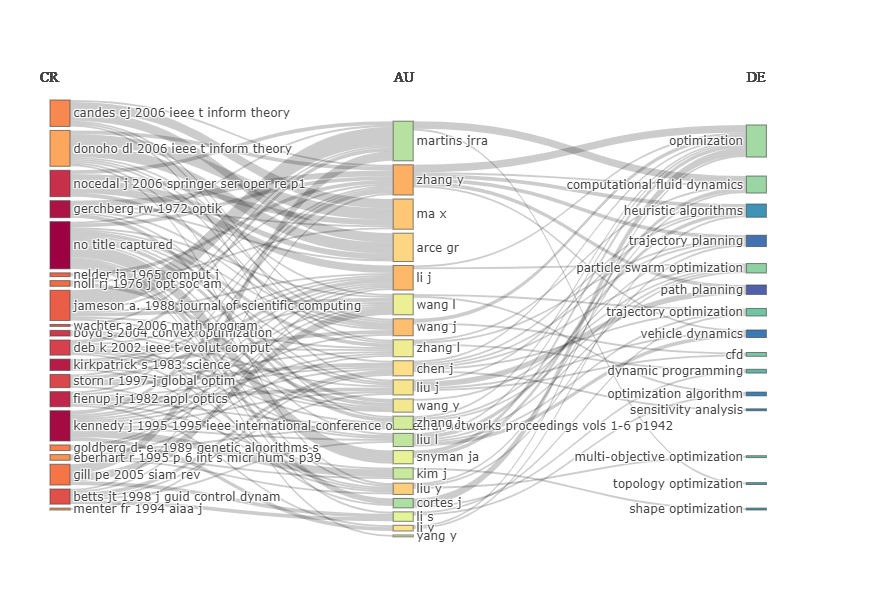
\includegraphics[width=1.3\textwidth]{experiments/KvotheKS/PesqBibliogr/AlgoritmosSimulacaoOptica-Dinamica/WoS-20220202/Dataset/AU_CR_DE.png}
    \caption{Dataset final}
    \label{fig:KvotheKS:Final_Data_Set}
\end{figure}

\subsection{Análise descritiva do \emph{dataset}}
    As informações iniciais do \emph{dataset} de 4859 registros são as seguintes:
    
\begin{description}
    \item [\textit{Timespan}] Todos os artigos que passaram pelo filtro e pela busca foram feitos de 1985 a 2022.
    \item [\textit{Sources (Journals, Books, etc)}] São 924 fontes de informação registradas.
    \item [\textit{Average years from publication}] A média de tempo para publicação é de 7,95 anos.
    \item [\textit{Average citations per documents}] A média de citações dos artigos é de 17,87 vezes.
    \item [\textit{Average citations per year per doc}] Os artigos, após sua publicação, tiveram em média 1,887 citações anuais.
    \item [\textit{References}] A quantidade total de referências do \emph{dataset} se dá em 127.349.
    \item [\textit{Keywords Plus (ID)}] 7.218 palavras-chave distintas foram encontradas no \emph{dataset}.
    \item [\textit{Author's Keywords (DE)}] 10.367 palavras-chave distintas escritas pelos autores.
    \item [\textit{Authors}] No total, foram 14.247 autores, sendo que boa parte deles tem origem chinesa.
    \item [\textit{Author Appearances}] No total, tiveram 20.024 aparições de autores, sendo que o número de autores distintos é, como mencionado anteriormente, 14.247
    \item [\textit{Authors of single-authored documents}] Dentre o número total de autores, apenas 206 fizeram pelo menos 1 artigo sozinhos.
    \item [\textit{Authors of multi-authored documents}] Se retirarmos do número total de autores, o número de autores que escreveram artigo(s) sozinhos, chegamos em 14.041 autores que escreveram apenas artigos coletivos.
    \item [\textit{Single-authored documents}] Dentro do \emph{dataset} apenas 227 deles são de criação individual.
    \item [\textit{Documents per Author}] Se dividirmos o número total de artigos pela quantidade de autores, chegamos em 0,341 artigos/autor.
    \item [\textit{Authors per Document}] Agora, inversamente se fizermos a quantidade de autores distintos divido pelo número de artigos, chegamos em 2,93 autores(/artigo.
    \item [\textit{Co-Authors per Documents}] Se pegarmos o número total de autores (também os repetidos) e dividirmos pela quantidade de documentos, temos 4.12 autores/artigo
    \item [\textit{Collaboration Index}] Por fim, a quantidade de vezes que autores distintos editaram artigos com um ou mais co-autores é de 3,03.
\end{description}
\subsection{Evolução da Produção Científica}
    Os temas procurados na busca são consideravelmente mais recentes que o esperado. O gráfico \ref{fig:KvotheKS:Annual_Scientific} mostra um crescimento quase que perfeitamente exponencial, sendo ele de 12.45\%.
    \begin{figure}[H]
    \centering
    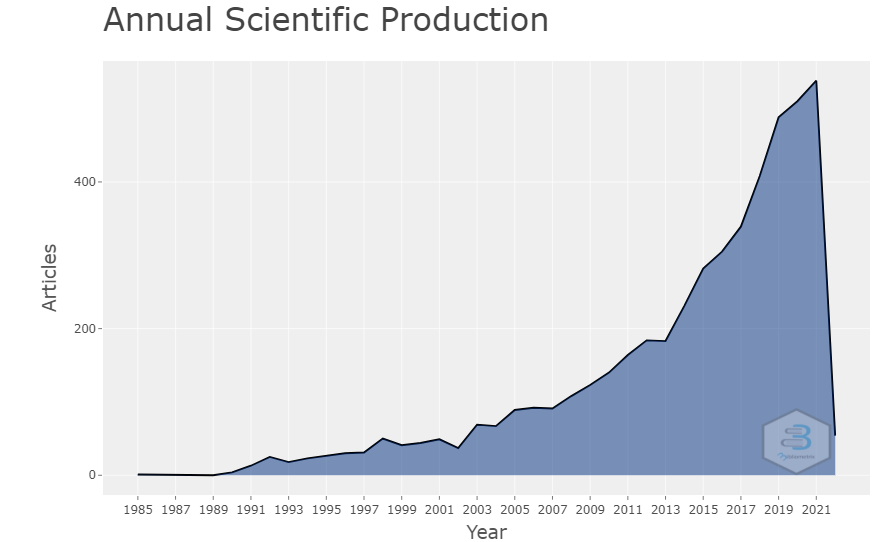
\includegraphics[width=1\textwidth]{experiments/KvotheKS/PesqBibliogr/AlgoritmosSimulacaoOptica-Dinamica/WoS-20220202/Dataset/Annual_Scientific.png}
    \caption{Produção anual científica}
    \label{fig:KvotheKS:Annual_Scientific}
\end{figure}
\subsection{Interpretação do crescimento}
    Com o avanço dos computadores e uma disponibilidade maior de recursos científicos como um todo, vários temas acabam ganhando força por fatores variados. No caso do meu \emph{dataset}, os estudos vão de análise topológica para robôs a estudo de aerodinâmica para aviões, e no fim acabam em simulações de iluminação.
\subsection{\emph{Clustering Network}}
    Como meio de demonstrar o quão "compacto" estão os resultados do \emph{dataset}, podemos utilizar uma \emph{Clustering Network}, que mostra em, em forma de grafo, quais estudos estão relacionados entre si, e qual peso de cada um.  
\begin{figure}[H]
    \centering
    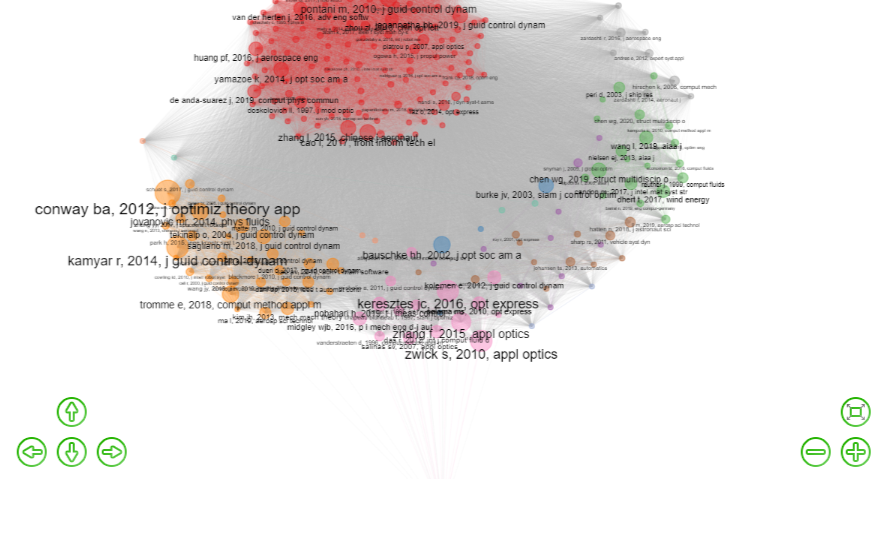
\includegraphics[width=1\textwidth]{experiments/KvotheKS/PesqBibliogr/AlgoritmosSimulacaoOptica-Dinamica/WoS-20220202/Dataset/Cluster_network.png}
    \caption{Grafo de citações}
    \label{fig:KvotheKS:Cluster_}
\end{figure}
\subsection{Interpretação da rede}
    Analisando a figura \ref{fig:KvotheKS:Cluster_}, podemos ver o quão inter-relacionados os artigos estão. Isso é um resultado óbvio do refinamento de dados feito anteriormente. Também mostra que alguns tópicos, como hidrodinâmica, aparecem em maior peso, por causa das revistas em qual artigos foram publicados. 
\subsection{\emph{Three-Field Plot}}
    Já foi demonstrado um dos \emph{Sankey diagrams} anteriormente \ref{fig:KvotheKS:Final_Data_Set}, onde o resultado mais interessante são as palavras-chave a direita, que mostram realmente quais são os tópicos mais abordados no \emph{dataset}. Porém alguns dados interessantes não foram abordados.
    
\begin{figure}[H]
    \centering
    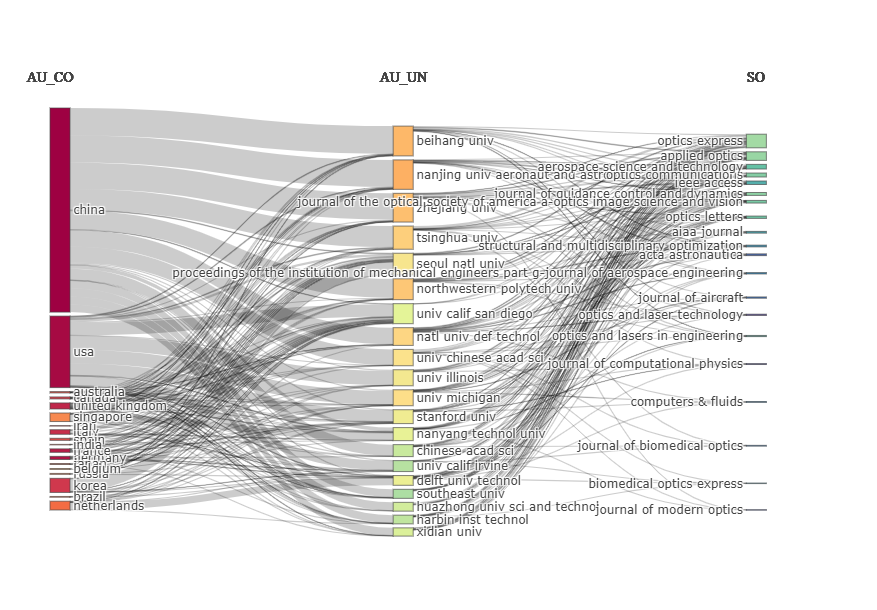
\includegraphics[width=1.1\textwidth]{experiments/KvotheKS/PesqBibliogr/AlgoritmosSimulacaoOptica-Dinamica/WoS-20220202/Dataset/AU_CO_AU_UN_SO.png}
    \caption{Afiliações, revistas e países}
    \label{fig:KvotheKS:SankeyCountry}
\end{figure}
\subsection{Considerações do peso dos países}
    Os dados interessantes da figura \ref{fig:KvotheKS:SankeyCountry} se dão nos países e universidades. Mais da metade dos artigos são chineses, porém não só há uma diversidade grande de universidades chinesas, mas também há uma falta de diferença entre as estado-unidenses, por onde artigos de vários países acabam passando.
\section{}